%%%%%%%%%%%%%%%%%%%%%%%%%%%%%%%%%%%%%%%%%%%%%%%%%%%%%%%%%%%%%%%%%%%%%%%%%%%%%%%%%%%%%%%%%%%%%%%%%%%%%%%%%%%%%%%%%%%%%%%%%%%%%%%%%%%%%%%%%%%%%%%%%%%%%%%%%%%
% This is just an example/guide for you to refer to when submitting manuscripts to Frontiers, it is not mandatory to use Frontiers .cls files nor frontiers.tex  %
% This will only generate the Manuscript, the final article will be typeset by Frontiers after acceptance.   
%                                              %
%                                                                                                                                                         %
% When submitting your files, remember to upload this *tex file, the pdf generated with it, the *bib file (if bibliography is not within the *tex) and all the figures.
%%%%%%%%%%%%%%%%%%%%%%%%%%%%%%%%%%%%%%%%%%%%%%%%%%%%%%%%%%%%%%%%%%%%%%%%%%%%%%%%%%%%%%%%%%%%%%%%%%%%%%%%%%%%%%%%%%%%%%%%%%%%%%%%%%%%%%%%%%%%%%%%%%%%%%%%%%%

%%% Version 3.4 Generated 2018/06/15 %%%
%%% You will need to have the following packages installed: datetime, fmtcount, etoolbox, fcprefix, which are normally inlcuded in WinEdt. %%%
%%% In http://www.ctan.org/ you can find the packages and how to install them, if necessary. %%%
%%%  NB logo1.jpg is required in the path in order to correctly compile front page header %%%

\documentclass[utf8]{frontiersSCNS} 
\usepackage{url,hyperref,lineno,microtype,subcaption,natbib}
\usepackage[onehalfspacing]{setspace}
\usepackage[english]{babel}
\usepackage{changes}
\usepackage{listings}
\definechangesauthor[name={George Chacko}, color=orange]{gc}
%\setremarkmarkup{(#2:#1)}
%\linenumbers
\usepackage{amsmath}
\usepackage{xcolor}
\usepackage{textcomp}

\newcommand\Tstrut{\rule{0pt}{2.9ex}} % "top" strut
\newcommand\Bstrut{\rule[-1.2ex]{0pt}{0pt}}   % "bottom" strut
\newcommand\TBstrut{\Tstrut\Bstrut} % "top and bottom" strut

% Leave a blank line between paragraphs instead of using \\

\def\keyFont{\fontsize{8}{11}\helveticabold }
\def\firstAuthorLast{Zhao {et~al.}} %use et al only if is more than 1 author
\def\Authors{Wenxi Zhao\,$^{1}$ and Dmitriy Korobskiy\,$^{1}$  and George Chacko\,$^{1,*}$} %Co-Author\,$^{2}$ 
% Affiliations should be keyed to the author's name with superscript numbers and be listed as follows: Laboratory, Institute, Department, Organization, City, State abbreviation (USA, Canada, Australia), and Country (without detailed address information such as city zip codes or street names).
% If one of the authors has a change of address, list the new address below the correspondence details using a superscript symbol and use the same symbol to indicate the author in the author list.
\def\Address{$^{1}$Netelabs, NET ESolutions (an NTT DATA Company), McLean, VA, USA}

% The Corresponding Author should be marked with an asterisk
% Provide the exact contact address (this time including street name and city zip code) and email of the corresponding author
\def\corrAuthor{George Chacko}


\def\corrEmail{netelabs@nete.com}
\begin{document}
\onecolumn
\firstpage{1}

\title[Delayed Co-citations]{Delayed Recognition; the Co-citation Perspective} 

\author[\firstAuthorLast ]{\Authors} %This field will be automatically populated
\address{} %This field will be automatically populated
\correspondance{} %This field will be automatically populated

\extraAuth{}% If there are more than 1 corresponding author, comment this line and uncomment the next one.
%\extraAuth{corresponding Author2 \\ Laboratory X2, Institute X2, Department X2, Organization X2, Street X2, City X2 , State XX2 (only USA, Canada and Australia), Zip Code2, X2 Country X2, email2@uni2.edu}

\maketitle

% ABSTRACT
\begin{abstract}
Enter abstract text later
\end{abstract}

\section{Introduction}

The term `Sleeping Beauty' has been used to describe an article that is not well cited in the early years after its publication but experiences a sharp increase in the rate at which it is subsequently cited~\citep{Raan2004}. One implication is that the new concept presented in such an article is `ahead of its time' and resistance to it delays recognition. Other causes for delayed recognition have also been postulated that include (i) information overload from the large amount of information available, (ii)  modest communication skills of authors, (iii) insufficient promotion of ideas, (iv) conflict with existing theory and experimental data, (v) the author's position in the social hierarchy of science, (vi)  multiple discovery, (vii) the management structures of scientific institutions, (viii), and the conservative nature of establishments~\citep{Barber1961,Merton1963,Cole1970,Garfield1970a,Garfield1980a}. The Sleeping Beauty phenomenon has been studied and debated with some degree of agreement that a fraction of the scientific literature exhibits citation kinetics that suggest delayed but eventual recognition of new ideas~\citep{Glanzel2003,Glanzel2004,Raan2004,redner_2005,Braun_2010,Li2014,Ke2015,Li2016,Song2018,sugimoto_mostafa_2018,ye_bornmann_2018,Raan2019}. 

Various approaches have been used to identify Sleeping Beauties and variants on this theme. Depth of sleep, length of sleep, and awake intensity as variables~\citep{Raan2004}, the Gini coefficient to examine later years of citation history~\citep{li_2014}, a parameter-free beauty coefficient ~\citep{Ke2015}, positional measures~\citep{costas2010}, and the citation angle by \cite{ye_bornmann_2018}. While earlier studies examined small datasets, subsequent ones considered large samples of the literature, for example, 22 million publications in \cite{Ke2015}.
	
The research referenced above has focused on single publications, however, new ideas also result from combining two previously independent ones, and the recognition of such novelty through recombination can be examined by co-citation analysis~\citep{MarshakovaShaikevich1973,Small1973,Uzzi2013,Boyack2014,Wang2017,Bradley2020}. Tracing co-citations, therefore, provides another lens with which to study delayed recognition. Measuring delayed recognition by co-citation has been briefly explored by ~\cite{devarakonda_2020} in a study of 33.6 million reference pairs. The authors used simplified criteria derived from prior Sleeping Beauty studies on single publications~\citep{Ke2015,Raan2004,Raan2019} and reported 24 co-cited pairs all in the 99th percentile of co-citation frequencies, and proposed the term \emph{delayed co-citations} for such cases. This initial exploration, albeit at scale, only considered reference pairs where each member of a pair was in the 99th percentile of highly cited articles in Scopus.   A somewhat related use of co-citation analysis is seen in \cite{zong_2018,teixeira2017sleeping} who sought to identify the so-called `princes' that awaken Sleeping Beauties. 

In this article, we extend the previous study on delayed co-citation to a much larger dataset, approximately 940 million pairs of articles. We refine the criteria in \cite{devarakonda_2020} and identify co-cited article pairs that exhibit delayed recognition using modifications of 
\cite{Raan2004,Raan2019} and  ~\cite{Ke2015}.  We also ask whether delayed co-citations are derived from Sleeping Beauty publications. 

\section{MATERIALS AND METHODS}

We have previously described a dataset of 33.6 million cited pairs each belonging to the top 1\% of cited articles in the Scopus bibliography~\citep[Figure~2]{devarakonda_2020}. In the present study, we include all co-cited pairs from references cited by articles published in Scopus in the 11 year period, 1985-1995, not only those drawn from the top 1\% of cited articles. We developed methods to handle a much larger volume of data using a combination of SQL, Cypher, and Python. Code for parsing Scopus XML data, a PostgreSQL schema for Scopus data, SQL, Cypher, and Python scripts used in this study are freely available from our Github repository~\citep{Korobskiy2019}.

To assemble and analyze a working dataset, we first exported 95,524,693 publication records from Scopus (all citation types) as a citation graph consisting of an edgelist and a nodelist, imported these data into a Neo4j database with publications as nodes with attributes and citations as edges. After creating indexes to improve performance, we selected all publications of citation type `article' published in the years 1985-1995 (inclusive of both), and that had at least five cited references each. In counting references, we only considered references with complete Scopus records and excluded any with cryptic placeholder identifiers. We further filtered rare cases in the data where a publication cites itself, or if the publication date of a cited reference was missing or greater than the publication date of its citing article. 

After initial comparison of SQL vs Cypher, we chose, on the basis of simplicity and performance, to use Cypher queries in Neo4j to generate all pairwise combinations, $n\choose 2$, of an article's cited references. We de-duplicated these pairs across all articles to assemble a dataset of 940 million pairs (940,357,633 pairs), roughly 28 times larger than the dataset in \cite{devarakonda_2020}. We then calculated the frequency of co-cited pairs by dividing the data and processing batches in parallel using Neo4j and the GNU Parallel utility.  After tuning experiments on a test set of 1 million pairs using a Neo4j 4.0 in a Centos 7.5 virtual machine with 128 Gb of RAM and 16 vCPUs in the Microsoft Azure environment, we set batch size to 1000 pairs and the degree of parallelization to 15 cores. Under these conditions, it took roughly 11 min to compute co-citation frequencies for a batch of 1,000 pairs. We then divided all 940 million pairs into 9 subsets of around 100 million pairs each and processed them at the rate of approximately 19 hours per subset. 

As an example, the simple Cypher query for calculating co-citation frequencies of pairs in Neo4j is shown below:
\lstset{language=Pascal, basicstyle=\footnotesize} 
\begin{lstlisting}[frame=single]
UNWIND $input_data AS row
MATCH (a:Publication{node_id: row.cited_1})<--(p)-->(b:Publication{node_id:row.cited_2})
RETURN row.cited_1 AS cited_1, row.cited_2 AS cited_2, count(p) AS scopus_frequency;
\end{lstlisting}

Frequencies thus calculated, were loaded back into PostgreSQL. For kinetic analysis, we selected all pairs with a co-citation frequency $>=$ 100 and calculated the kinetics of citation accumulation from the first possible year of co-citation for each pair through the year 2018, again in Neo4j.  Finally, for continuity of coverage, we set zero as frequency for all missing years between the first possible year of co-citation and the last co-cited year (2018). Minor differences between the data in  \cite{devarakonda_2020} are on account of more current data in Scopus and computing kinetic data through 2018 in this study. We compared small samples between the two datasets and found that minor differences in co-citation frequencies could be bridged by including citations from publications in 2019 and later. 

\textcolor{blue}{For Wenxi}
\emph{Identifying Sleeping Beauty publications}

\emph{Identifying Delayed Co-citations}

\emph{Calculating slope}

\emph{Calculating the Beauty Coefficient for Publications and Co-cited Pairs}

\section{RESULTS AND DISCUSSION}

In this study on delayed co-citations, we first examined cited references in 3,433,578 publications in the Scopus database that were published in the years 1985-1995. The criteria for selection of these publications were that they were classified as `article', that they were published in the period 1985-1995, and they contained at least 5 cited references each. We generated all possible co-cited pairs for the references in these articles and de-duplicated them since the same reference pair can occur in more than one article. Then we measured the co-citation frequency of each pair across the entire Scopus database by counting all co-citation events from the first possible year onwards(Fig \ref{fig:fig1},Table \ref{tab:table1}).

\iffalse
of co-citation through 2018 (Fig \ref{fig:fig1},Table \ref{tab:table1}). The distribution of co-citation frequencies mirrors an earlier report~\citep{devarakonda_2020}, in which we describe a combination of lognormal and power law distributions. [We need to say some more about this huge undertaking].
\fi

\begin{figure}[h!]
\begin{center}
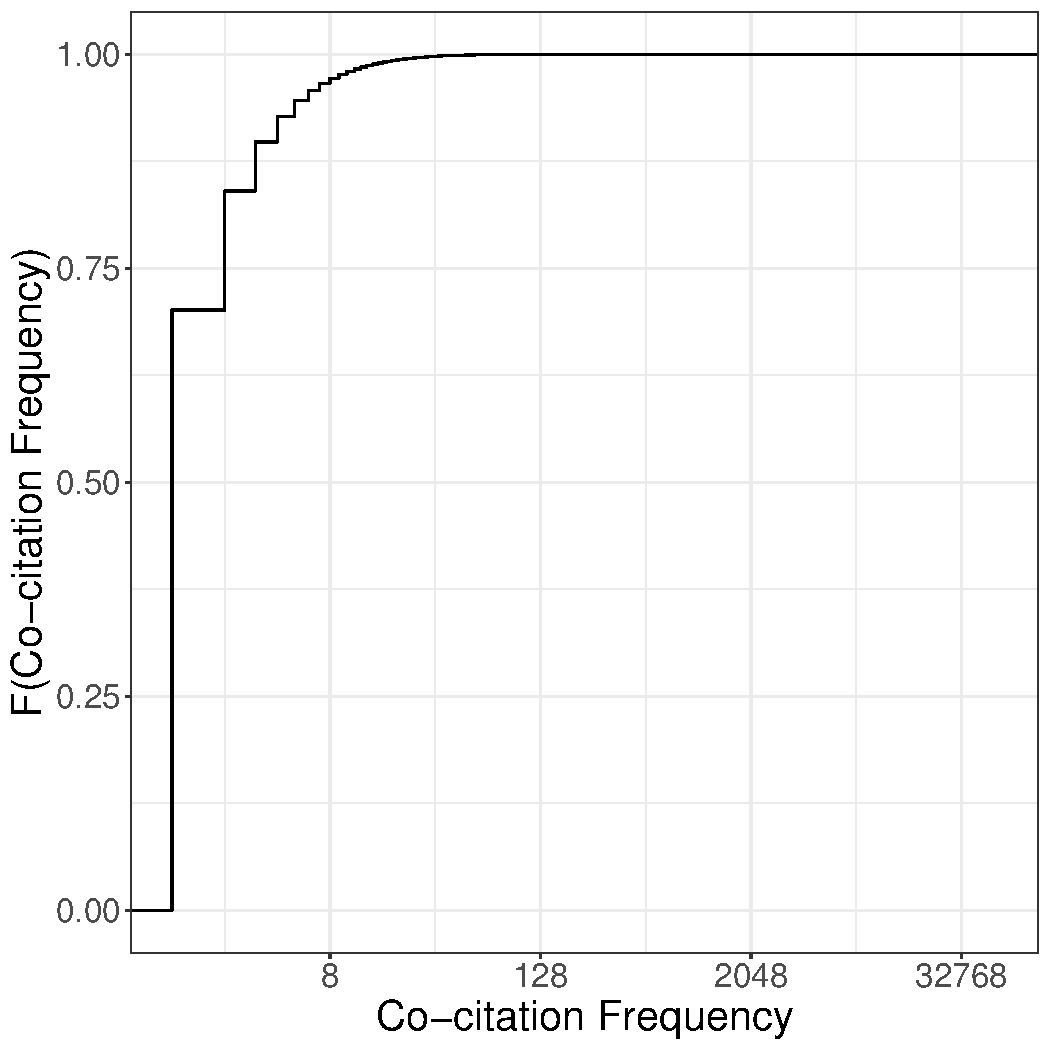
\includegraphics[width=10cm]{fig1}% This is a *.eps file
\end{center}
\caption{Frequencies of $\sim$940 million co-cited pairs drawn from Scopus 1985-1995. Pairwise combinations, $n\choose 2$, of references from articles indexed in Scopus (1985-1995), were generated as described in Materials and Methods. Total co-citation frequencies for these pairs, ranged from 1 to 52,471 with a median frequency of 1. The empirical cumulative distribution function (ECDF) was calculated from 940,357,633 co-citation frequencies and plotted against co-citation frequencies on a log\textsubscript{2} scale using the ggplot2 package and the expression \emph{ggplot(x, aes(frequency) + stat\_ecdf(geom=\textquotesingle step\textquotesingle)}}
\label{fig:fig1}
\end{figure}

\begin{table}[ht]
\caption{Distribution of ~940 million Co-citation Frequencies. The count of co-cited pairs in each frequency class as well as the percentage relative to the total number of 940,357,633 is shown. Counts include the lower bound in each class and exclude the upper bound. Add legend details}% title of Table
\centering % used for centering table
\begin{center}
\begin{tabular}{rll} 
\emph{f} Interval & Count & Percentage \\
\hline % inserts single horizontal line\
$<=$ 2 & 790,189,114 & 84.03 \Tstrut\\ 
2 -4 & 82,022,893 & 8.72 \\
4 -8 & 41,772,728 & 4.44 \\
8 -16 & 17,749,436 & 1.89 \\
16-32 & 6,429,234 & 0.68\\
32-64 & 1,704,908 & 0.18\\
64-128 & 385,923 & 0.041\\
128-256 & 81,164 & 0.0086\\ 
256-512 & 17,150 & 0.0018\\
512-1024 & 3,777 & 0.00040\\
1024-2048 & 948 & 0.00010\\ 
$> $ 2048 & 358 & 0.000038\\   
\hline 
\end{tabular}
\end{center}
\label{tab:table1} % is used to refer this table in the text
\end{table}


The data in Fig \ref{fig:fig1} show a highly skewed distribution of co-citation frequencies across a large dataset. Roughly 84\% of the pairs have a total co-citation frequency of 2 or less, and the 99th percentile is 16 although each pair had at least 10 years to accumulate co-citations. Even for a pair of articles from the most recent year in our data, 1995, this frequency of 16 corresponds to less than one co-citation per year on average. Thus, only a small fraction of pairs in these data have co-citation frequencies greater than 2 per year. One must consider that the reasons advanced for delayed recognition described in the Introduction could also extend to non-recognition of merit and a recognition of non-merit.

Beyond a high level understanding of the distribution of co-citation frequencies, however, we are interested in frequently co-cited publications, which represent a high degree of interest from the community, and are derived from highly cited publications~\citep{Small1973}. Thus, we subset the data using a more intuitive threshold of 100 for co-citation frequency along with a maximum annual co-citation frequency of at least 20. These criteria are analogous to those proposed by van Raan~\citep{Raan2004} and Redner~\citep{redner_2005}. After applying these two further restrictions, the number of co-cited pairs is reduced to 51,613 (approximately 0.055\% of the total number of pairs).

To find cases of delayed co-citation, we applied the following conditions to these 51,613 pairs: (i)  A co-cited paper should have slept for at least $10$ years and received no more than $2$ co-citations in each year during this sleeping period, which is defined as as the number of years from the first possible co-cited year to the first year that the pair receives more than $2$ co-citations. During this sleeping period, the average annual co-citation frequency $<=$1 and the maximum allowed annual co-citation frequency is 2. To be considered as a sleeping beauty, the awakening period that follows the sleeping period is characterized by (i) a peak annual co-citation frequency of $>=$20 and a minimum total frequency of 100. The above criteria when collectively applied, identified 1,196 cases of delayed co-citation, which are summarized in Table \ref{tab:table2}. We also calculated the slope between the co-citation frequency in the first awakening year and the peak frequency and noted 10 cases where the maximum possible slope was seen Table \ref{tab:table3}. We have previously modified the Beauty Coefficient~\citep{Ke2015}, which was designed to measure kinetics in single publications, to be useful to the case of co-cited pairs~\citep{devarakonda_2020} and we computed it for these 1,196 pairs observing a range of 34.21-1678.62. These data are collectively summarized in Table \ref{tab:table2}.  

\begin{table}[ht]
\caption{Summary Statistics of 1196 Delayed Co-citation Pairs. Insert stuffer text here}% title of Table
\centering % used for centering table
\begin{center}
\begin{tabular}{rllll} 
& Total Frequency & Sleep Duration & Slope & Mod. Beauty Coefficient* \\
\hline % inserts single horizontal line
Min &  20.00 & 10.00 & 0.21 & 34.21   \Tstrut\\ 
Q1  &  22.00 & 11.00  & 1.23 & 89.40   \\ 
Median & 26.00 & 14.00 & 1.7000 & 128.53   \\ 
Mean & 34.06 & 15.11 & 2.40 & 167.63   \\ 
3rd Qu & 36.00 & 17.00 & 2.67 & 190.93   \\ 
Max & 296.00 & 38.00  & 38.00  & 1678.62   \\ 
\hline
\end{tabular}
\end{center}
\label{tab:table2} % is used to refer this table in the text
\end{table}

Interestingly. these 1,196 pairs are derived from only 1,267 of a possible 2,392 individual publications indicating that some members of frequently co-cited pairs are found in multiple pairs. Indeed, we have previously noted that a pair of articles concerning methods in biochemistry, contribute to over 40,000 different co-cited pairs of frequency $>=$ 10~\citep{devarakonda_2020}.  Secondly, in contrast to co-citation frequencies for delayed co-citations (Fig. \ref{tab:table2}), which range from 20-260; citation counts for the 1,267 publications that contribute to these 1196 delayed co-citations range from 121 to 190,832 with 72 of these publications having citation counts of $>$10,000. However, co-cited pairs do exceed the seemingly modest frequencies noted for delayed co-citations. For example, a pair of articles from the field of physical chemistry published in 1993, and 1988 have been co-cited over 51,000 times but does not exhibit delayed citation kinetics. Similarly, 1,357 pairs from the data shown in Fig \ref{fig:fig1} have co-citation frequencies greater than 1,000.
What becomes clear is that delayed co-citations tend to have frequency profiles that are lower than those of single publications. This is not unexpected since co-cited frequencies cannot exceed the citation frequencies of the publications in these pairs but it does suggest that seemingly low co-citation frequencies should not be overlooked on account of low amplitude signal. Of the 1196 delayed co-citations, the slope could not be computed for 10 pairs because the peak year was the year of awakening, implying sudden recognition, during awakening, of the concepts represented by these pairs (Table \ref{tab:table3}. These 10 span the areas of LED technology, cosmology, immunology, psychology, and computational science. One publication from 1985 titled, ``An exotic class of Kaluza-Klein models" appears in 3 of 10 pairs and the author himself refers, 1999, to `renewed interest due to the explosion of activity in the non compact extra dimensions variant of the Kaluza Klein model'~\citep{visser_1999}.

\begin{table}[ht]
\caption{10 pairs that have maximum slope at the first year of awakening}% title of Table
\centering % used for centering table
\begin{center}
\begin{tabular}{ll} 
\hline % inserts single horizontal line
PubYears & Title \\
\hline 
\tiny{1974} & \tiny{Fundamental energy gap of GaN from photoluminescence excitation spectra} \Tstrut\\
\tiny{1971} &  \tiny{Absorption, reflectance, and luminescence of GaN epitaxial layers} \\
\hline
\tiny{1986} & \tiny{Dimensional reduction caused by a cosmological constant} \\
\tiny{1985} & \tiny{An exotic class of Kaluza-Klein models} \\
\hline
\tiny{1987} & \tiny{Spacetime as a membrane in higher dimensions} \\
\tiny{1985} & \tiny{An exotic class of Kaluza-Klein models} \\
\hline 
\tiny{1985} & \tiny{An exotic class of Kaluza-Klein models} \\
\tiny{1985} & \tiny{Do we live inside a domain wall?} \\
\hline
\tiny{1971} & \tiny{Mental rotation of three-dimensional objects} \\
\tiny{1976} & \tiny{Demonstration of a mental analog of an external rotation} \\
\hline
\tiny{1974} & \tiny{Biologic and clinical significance of cryoglobulins. A report of 86 cases} \\
\tiny{1980} & \tiny{Mixed cryoglobulinemia: Clinical aspects and long-term follow-up of 40 patients} \\
\hline
\tiny{1977} & \tiny{Imitation of Facial and Manual Gestures by Human Neonates} \\
\tiny{1979} & \tiny{Matching behavior in the young infant.} \\ 
\hline
\tiny{1978} & \tiny{Cognitive determinants of fixation location during picture viewing} \\
\tiny{1979} & \tiny{Framing pictures: The role of knowledge in automatized encoding and memory for gist} \\
\hline
\tiny{1983} & \tiny{Parst: A system of fortran routines for calculating molecular structure parameters (truncated)} \\
\tiny{1983} & \tiny{On enantiomorph‐polarity estimation} \\
\hline
\tiny{1980} & \tiny{Toward a positive theory of consumer choice} \\
\tiny{1973} & \tiny{On the psychology of prediction} \\
\hline 
\end{tabular}
\end{center}
\label{tab:table3} % is used to refer this table in the text
\end{table}

A logical question is whether any of these 1,267 individual publications would be classified as Sleeping Beauties. Applying van Raan's criteria (\textcolor{blue}{@Wenxi} Materials and Methods), we identify 128 of these 1,267 publications as Sleeping Beauties. Interestingly, 27 pairs were cases where both members were Sleeping Beauties. Of these, the 1978 article by Rassias titled `On the stability of the linear mapping in Banach spaces' was a member of four different pairs. Thus, delayed recognition can occur without a requirement that at least one member of a co-cited pair with delayed recognition should have Sleeping Beauty characteristics. These  observations also suggest that while high-referencing fields such as biology~\citep{Small1980} might be advantaged by our selection criteria, the thresholds we set do not entirely exclude other fields. Nevertheless, extending this work with field normalization of co-citation frequencies is warranted.

To ask which fields these 1,196 delayed co-citations are found in, we mapped them to the All Science Journal Classification (ASJC) maintained by Scopus, which consists of XX categories.  The data are represented in Figure \ref{fig:fig2} but should be interpreted in the light of the labels being assigned to journals rather than articles and that an article may have more than one label. 


\begin{figure}[h!]
\begin{center}
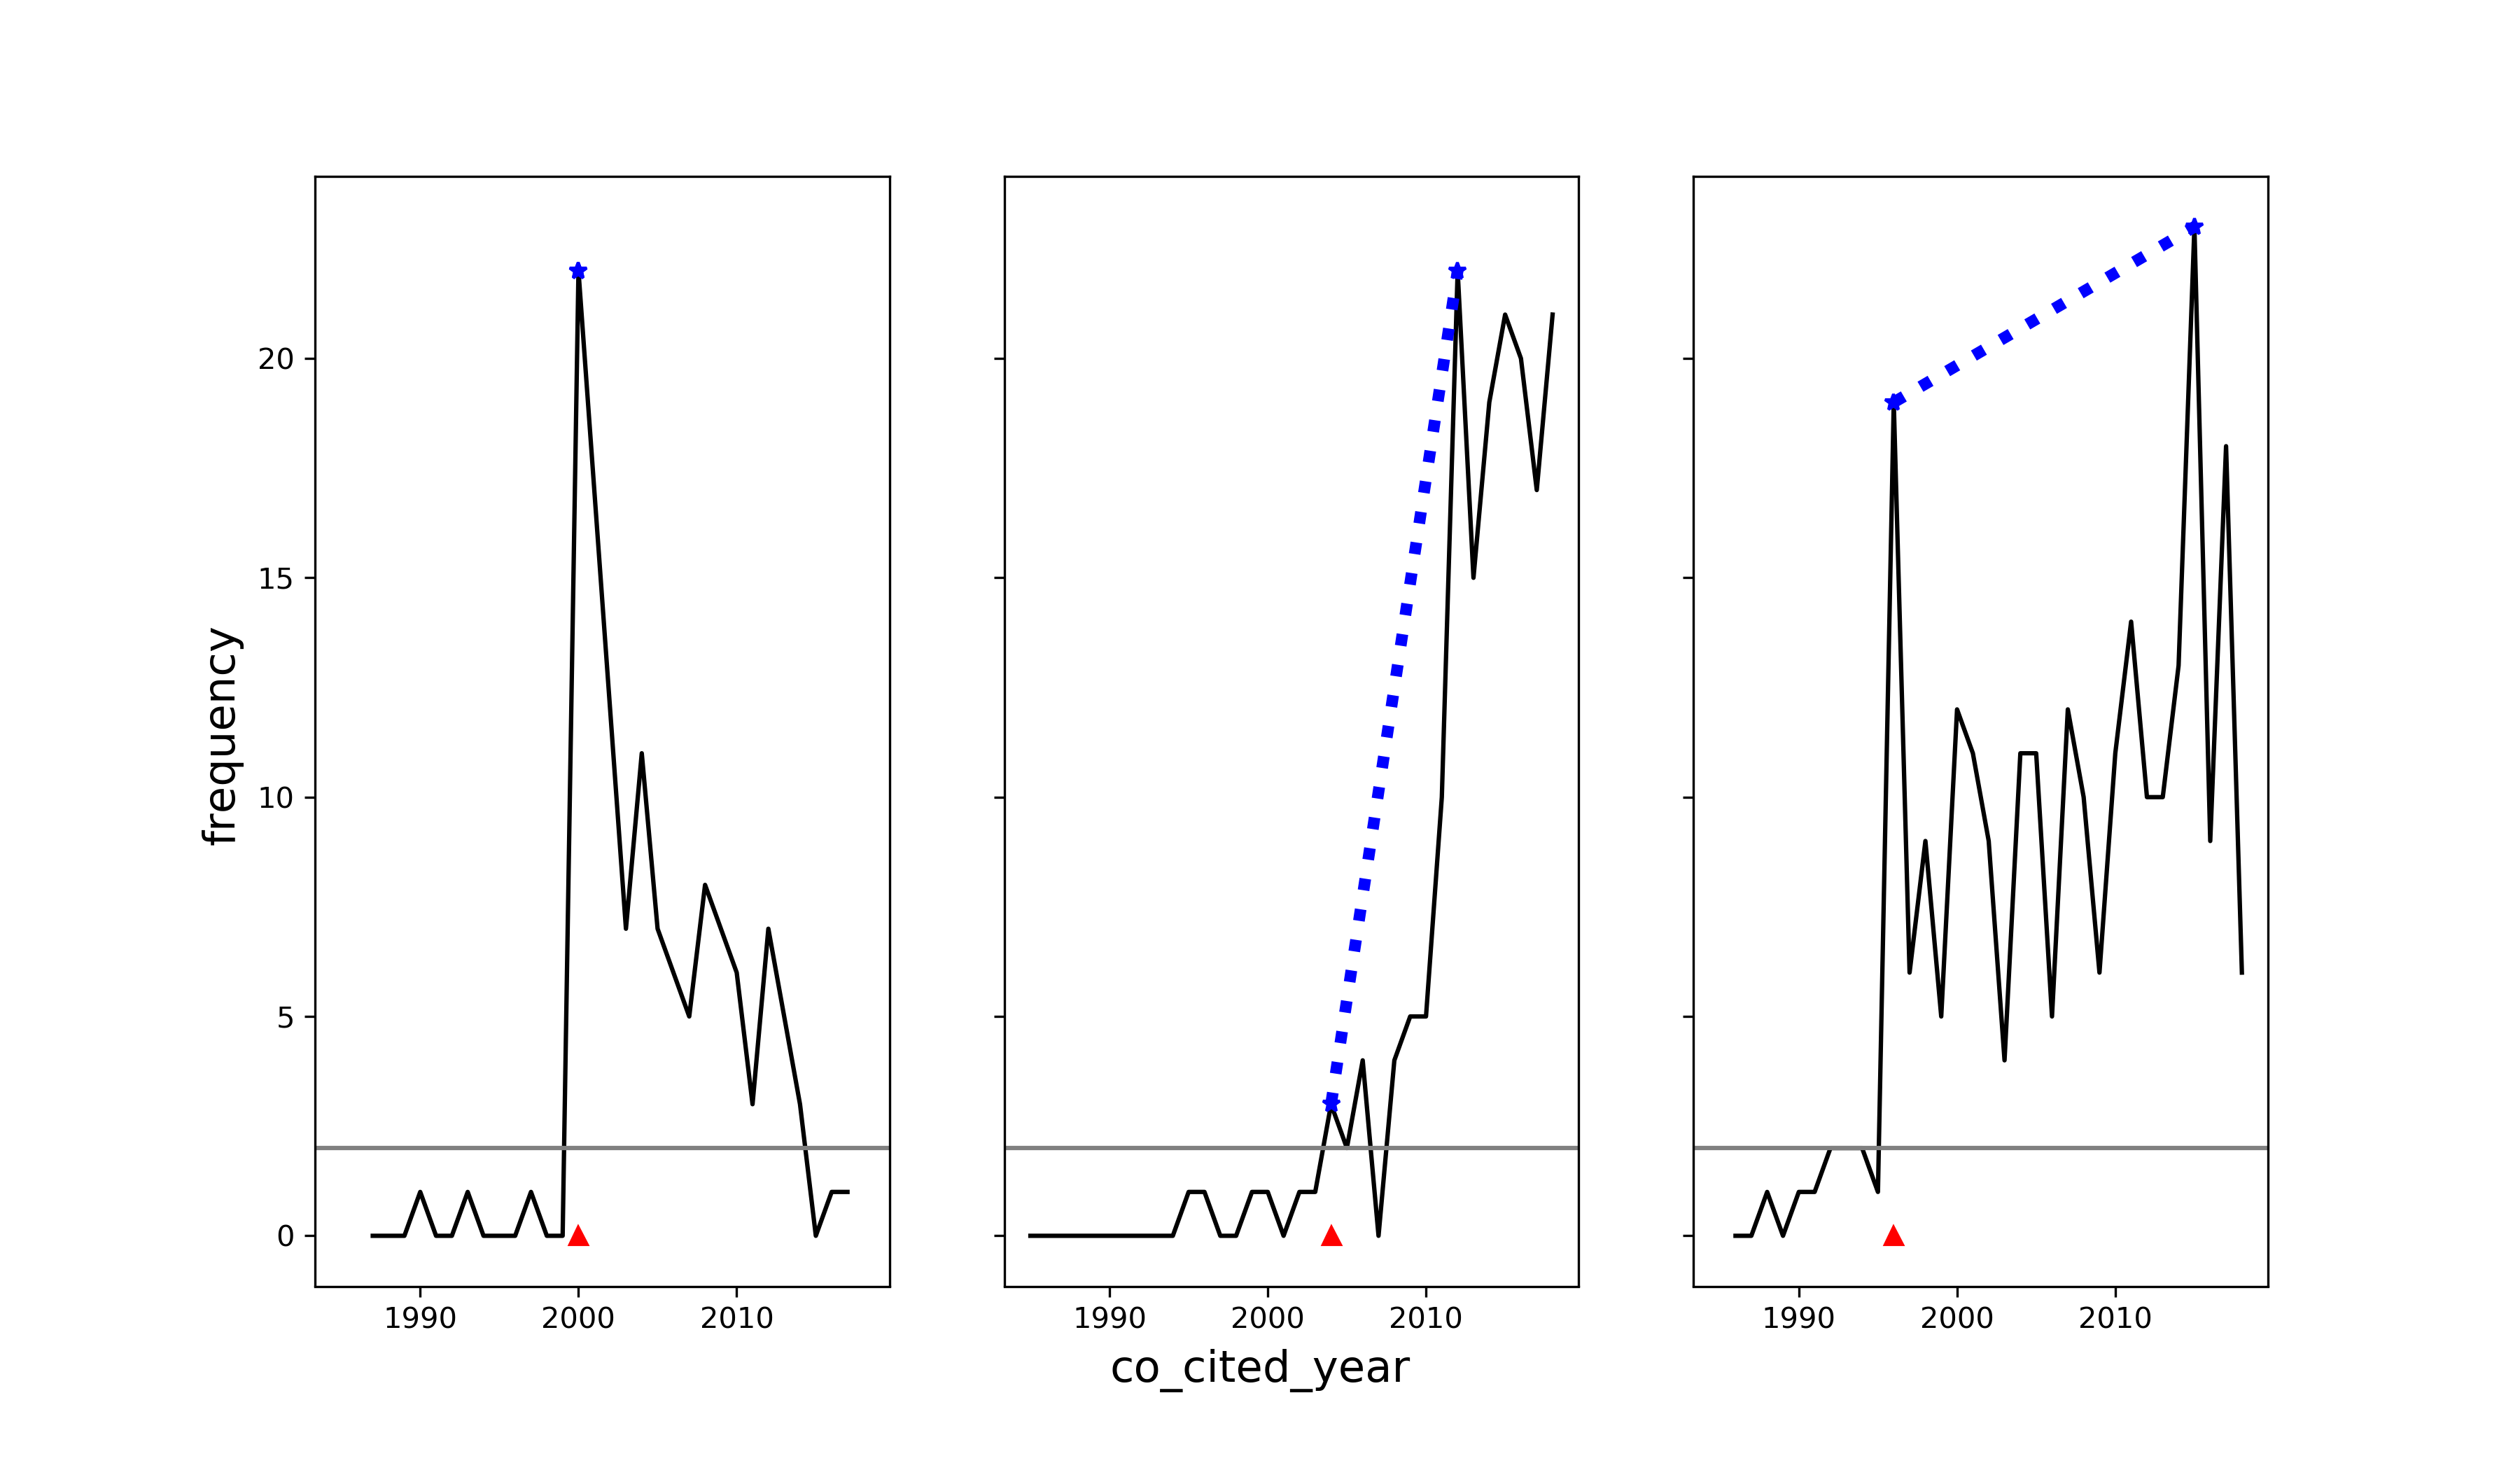
\includegraphics[width=10cm]{fig2}% This is a *.eps file
\end{center}
\caption{We need a meaningful caption and one sentence. Each node represents a major subject are in the Scopus ASJC classification. Major subject areas are abbreviated in the graphic:
\emph{MTH} (Mathematics);
\emph{IMM} (Immunology and Microbiology);
\emph{HP} (Health Professions);
\emph{GEN} (General);
\emph{ENS} (Environmental Science);
\emph{ENG} (Engineering);
\emph{EPS} (Earth \& Planetary Sciences);
\emph{DCS} (Decision Sciences);
\emph{MAT} (Material Sciences);
\emph{CEN} (Chemical Engineering);
\emph{PSY} (Psychology);
\emph{PHY} (Physics and Astronomy);
\emph{NEU} (Neuroscience);
\emph{CS}( Computer Science);
\emph{A\&H} (Arts and Humanities);
\emph{SS} (Social Sciences);
\emph{MED} (Medicine);
\emph{CHE} (Chemistry);
\emph{ABS} (Agricultural \& Biological Sciences); 
\emph{BGMB} (Biochemistry, Genetics \& Molecular Biology);
\emph{BMA} (Business, Management, and Accounting);
\emph{EEF} (Economics, Econometrics and Finance)
\emph{PTP} (Pharmacology, Toxicology \& Pharmaceutics)}
\label{fig:fig2}
\end{figure}

 [Now is the time to critique Ke. Why did we pick BC and not the awakening time criteria. They do not provide a threshold value- therefore we applied positional measures].



\begin{table}[ht]
\caption{Statistical Summary of Slope for 1196 Delayed Co-citation pairs}% title of Table
\centering % used for centering table
\begin{center}
\begin{tabular}{cll} 
\hline % inserts single horizontal line
count & 870 \\
mean & 2.38 \\
std & 2.36 \\
min & 0.44 \\
25\% & 1.25 \\
50\% & 1.71 \\
75\% & 2.69 \\
max & 38 \\
\hline 
\end{tabular}
\end{center}
\label{tab:table4} % is used to refer this table in the text
\end{table}

\section{CONCLUSION} In a large-scale exploration of the kinetics of co-citation, we 

\section{Additional Requirements}

For additional requirements for specific article types and further information please refer to \href{http://www.frontiersin.org/about/AuthorGuidelines#AdditionalRequirements}{Author Guidelines}.

\section*{Conflict of Interest Statement}
%All financial, commercial or other relationships that might be perceived by the academic community as representing a potential conflict of interest must be disclosed. If no such relationship exists, authors will be asked to confirm the following statement: 

The authors declare that the research was conducted in the absence of any commercial or financial relationships that could be construed as a potential conflict of interest.

\section*{Author Contributions}

The Author Contributions section is mandatory for all articles, including articles by sole authors. If an appropriate statement is not provided on submission, a standard one will be inserted during the production process. The Author Contributions statement must describe the contributions of individual authors referred to by their initials and, in doing so, all authors agree to be accountable for the content of the work. Please see  \href{http://home.frontiersin.org/about/author-guidelines#AuthorandContributors}{here} for full authorship criteria.

\section*{Funding}
Details of all funding sources should be provided, including grant numbers if applicable. Please ensure to add all necessary funding information, as after publication this is no longer possible.

\section*{Acknowledgments}
This is a short text to acknowledge the contributions of specific colleagues, institutions, or agencies that aided the efforts of the authors.

\section*{Supplemental Data}
 \href{http://home.frontiersin.org/about/author-guidelines#SupplementaryMaterial}{Supplementary Material} should be uploaded separately on submission, if there are Supplementary Figures, please include the caption in the same file as the figure. LaTeX Supplementary Material templates can be found in the Frontiers LaTeX folder.

\section*{Data Availability Statement}
Data used in this study are restricted by a license from Elsevier Inc. Interested persons with a license can use the code on our Github repository to reproduce these findings by recreating the source data, our schemata, and the results of this work.

%%% Make sure to upload the bib file along with the tex file and PDF
%%% Please see the test.bib file for some examples of references
\bibliographystyle{frontiersinSCNS_ENG_HUMS} 
\bibliography{sb}

\section*{Figure captions}

\end{document}

%%% Please be aware that for original research articles we only permit a combined number of 15 figures and tables, one figure with multiple subfigures will count as only one figure.
%%% Use this if adding the figures directly in the manuscript, if so, please remember to also upload the files when submitting your article
%%% There is no need for adding the file termination, as long as you indicate where the file is saved. In the examples below the files (logo1.eps and logos.eps) are in the Frontiers LaTeX folder
%%% If using *.tif files convert them to .jpg or .png
%%%  NB logo1.eps is required in the path in order to correctly compile front page header %%%

\begin{figure}[h!]
\begin{center}

\includegraphics[width=10cm]{logo1}% This is a *.eps file
\end{center}
\caption{ Enter the caption for your figure here.  Repeat as  necessary for each of your figures}\label{fig:1}
\end{figure}

\begin{figure}[h!]
\begin{center}
\includegraphics[width=15cm]{logos}
\end{center}
\caption{This is a figure with sub figures, \textbf{(A)} is one logo, \textbf{(B)} is a different logo.}\label{fig:2}
\end{figure}

%%% If you are submitting a figure with subfigures please combine these into one image file with part labels integrated.
%%% If you don't add the figures in the LaTeX files, please upload them when submitting the article.
%%% Frontiers will add the figures at the end of the provisional pdf automatically
%%% The use of LaTeX coding to draw Diagrams/Figures/Structures should be avoided. They should be external callouts including graphics.

\end{document}

{We report that...}{Sleeping Beauty in scientific community refers to a single well-cited article which receives delayed recognition because of being ahead of time or overlooked for periods. Anthony F.J. van Raan and other researchers have proposed different methods to identify Sleeping Beauty articles and measure their kinetics. This phenomenon also happens for co-cited pairs that a pair of publications have been cited by one or more publications together. The more often a pair of publications has been co-cited, the more related they are assumed to be https://arxiv.org/pdf/1707.03076.pdf. The appearance of Sleeping Beauty among co-cited pairs indicates that as time goes on, different disciplines gradually have overlaps or different ideas have been combined and evolved into a new concept. In our experiment, we extend to examine Sleeping Beauty phenomenon for highly co-cited pairs that have been sunk in sleep for a long period before attracting citations, propose an approach to define Sleeping Beauty among co-cited pairs and investigate the kinetics of Sleeping Beauty co-cited pairs and their individual articles. To find possible Sleeping Beauty co-cited pairs, we constructed a dataset of articles from Scopus (Elsevier BV, 2019) by extracting co-cited pairs which were composed of highly co-cited individual articles and have received at least 10 co-citations. We assembled 4.12 million co-cited pairs as a result. We developed an initial method to find possible Sleeping Beauty co-cited pairs within our dataset, and in order to further investigate kinetics of those possible Sleeping Beauty co-cited pairs, we built another dataset of individual articles from filtered co-cited pairs. To determine the number of Sleeping Beauty individual articles found in this dataset, we applied modified van Raan's procedures to filter out articles by setting the most stringent constraints and then calculated the beauty coefficient proposed by Ke et al. Then by calculating the number of Sleeping Beauty individual articles that each filtered co-cited pairs has and adjusting the constraints we applied, we answered the question that does it take at least one Sleeping Beauty individual article to generate a Sleeping Beauty co-cited pair. Lastly, we also investigated edge cases that a co-cited pair awaked after a long period of dormancy and then fell asleep again. We proposed a new method to define such Sleeping Beauty individual articles, since both van Raan's and Ke's method were not applicable in such cases, and defined them as unstable Sleeping Beauties.}

Detection of Sleeping Beauties has largely followed a parameterized and parameter free formulations...not sure how to say this but I need to introduce the Beauty Coefficient somehow.

Ke et al proposed Beauty Coefficient B to quantify how much a given paper can be considered as an SB~\citep{Ke2015}. Given a publication, Ke defines $c\textsubscript{0}$ as the number of citations received in the year of publication and $c\textsubscript{t}$ as the number of citations received in each year after the year of publication, where $t$ indicates the number of years. The reference line of a publication is defined as a straight line $l\textsubscript{t}$ that connects the start point $(0, c\textsubscript{0})$ and peak point $(t\textsubscript{m}, c\textsubscript{t\textsubscript{m}})$ where $m$ indicates that at the age of $t\textsubscript{m}$ the paper receives its maximum number of citations $c\textsubscript{t\textsubscript{m}}$. Then this line $l\textsubscript{t}$ can be described by the equation:
\begin{equation}
\l\textsubscript{t} = \frac{c\textsubscript{t\textsubscript{m}} - c\textsubscript{0}}{t\textsubscript{m}} \times t + c\textsubscript{0}
\end{equation}
where $t \in [t\textsubscript{0}, t\textsubscript{m}]$ and ${c\textsubscript{t\textsubscript{m}} - c\textsubscript{0}}/{t\textsubscript{m}}$ is the slope of the reference line. Then for each $t$, first compute difference between the reference line l\textsubscript{t} and the citation history of the paper c\textsubscript{t}, and second compute the ratio between this difference and $max\{1, c\textsubscript{t}\}$. By summing up this ratio for each $t$, the Beauty Coefficient B is defined as:
\begin{equation}
B = \sum_{t = 0}^{t\textsubscript{m}} \frac{\frac{c\textsubscript{t\textsubscript{m}} - c\textsubscript{0}}{t\textsubscript{m}} \times t + c\textsubscript{0} - c\textsubscript{t}}{max\{1, c\textsubscript{t}\}}
\end{equation}

\begin{figure}
\begin{center}
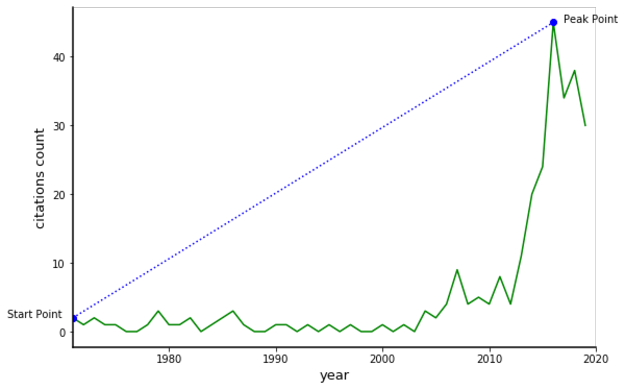
\includegraphics{Picture1}
\caption{for this figure to be useful, it needs to have additional features. Demonstration of Ke's Beauty Coefficient (Eq. 2). (We can discuss whether we should add anything to this plot based on the defects I stated below, or cite it directly from Ke, or just remove it) You also need to reference the modification to Ke that we did in Sitaram's paper.}
\label{fig:1} 
\end{center}
\end{figure}

On  \textbf{Figure 1}, The green curve represents the number of citations c\textsubscript{t}that a paper received at each year and $t$ is the number of years between two years. The blue dotted line represents the reference line, which connects the peak point $(t\textsubscript{m}, c\textsubscript{t\textsubscript{m}})$ and start point $(0, c\textsubscript{0})$. This Beauty Coefficient B can be computed for any paper and does not rely on arbitrary selections of parameters such as length of sleeping period and awakening intensity. A paper who have a linear kinetics with time $c\textsubscript{t} = l\textsubscript{t}$ will have Beauty Coefficient $B = 0$, and thus if a paper can be considered as Sleeping Beauty, it must have a positive Beauty Coefficient, which means its kinetics is a concave function of time. Further, this equation penalizes earlier citations since the summation of ratio in earlier years will be much less than the one in later years when the number of citations received is the same, and so with longer sleeping period, larger maximum citations received, and more abrupt changes happened before the maximum number of citations reached, a publication will have a larger Beauty Coefficient B. 

\emph{This is the best part of the paper- written like a scientist!- although it still needs more work}
But Ke's method also has three major defects: (i) This approach doesn't put any constraints on any parameters. In general, a paper who has very large Beauty Coefficient B will have a long sleeping period, abrupt changes in citations received before reaching the peak point, and a very high peak point. But in extreme cases, as long as the peak point is high enough, a paper will definitely have a larger B value. For example, if a paper published in $2014$ receives $3000$ citations in $2018$, then even though the sleeping period is only $3$ years and each year receives only $2$ citations, by (Eq. 2) the Beauty Coefficient B equals to $2998$, which is large enough for a paper to be identified as Sleeping Beauty(Ke et al lists top 15 Sleeping Beauties in science and all of those papers have Beauty Coefficient B larger than 2000~\citep{Ke2015}). The paper in such extreme case apparently shouldn't be considered as Sleeping Beauty, which also proves that a paper must have a large positive Beauty Coefficient to be identified as Sleeping Beauty, but a paper with large positive Beauty Coefficient is not necessarily a Sleeping Beauty. (ii) Ke et al mentions that Sleeping Beauty papers will have a large Beauty Coefficient B, but he doesn't provide a exact threshold to define how large a Beauty Coefficient B should a paper have to be a Sleeping Beauty. When he examines interdisciplinary nature of top Sleeping Beauties, he divides papers into three disjoint subsets with high, medium, and low values of Beauty Coefficient B, which is the group of top $1000$ SBs $(B \geq 317.93)$, the $1001st$ to the top $1\%$ SBs $(33.21 \leq B \leq 317.93)$, and the rest $(B \leq 33.21)$~\citep{Ke2015}). These cutoff values are quite arbitrary and cannot be directly applied to other datasets. Thus the application of this Beauty Coefficient is quite unclear. (iii) Ke et al does not consider the citations received after the peak point is reached. Since Sleeping Beauty papers are those who have delayed recognization, in most cases they will keep sleeping in earlier years, gradually gain citations and reach the peak point in recent years. But this doesn't mean that we can completely ignore the kinetics after the peak point is reached. The biggest problem it will cause is that when a paper reaches its peak point twice, how should this reference line be drawn? Should we connect the start point to the first peak point or the second peak point? What if there are more than two peaks? Further, if a paper reaches its peak point in its publication year, and goes back to sleep for several years and wake up again, should we ignore all those kinetics since the start point equals to the peak point and the reference line could not be drawn? We'll further explore this kine of edge case later. 

van Raan proposed another totally different method to identify Sleeping Beauties. He tuned four main parameters: (1) length of sleeping period; (2) depth of sleep, in terms of the citation rate during sleeping period; (3) awakening period, which is $5$ years after sleeping period; (4) awakening citation-intensity in terms of the citation rate during awakening period~\citep{Raan2019}). van Raan focused on investigating the number of SBs identified with different combinations of parameters, especially with different length of sleeping period, and deriving the general 'General Sleeping Beauty Equation' to gives the number of SBs identified depend on those parameters. 

In our experiment, we made minor adjustments to this method. Based on initial limitations we set on our Sleeping Beauty co-citation pairs, we also required individual papers to have slept for at least $10$ years. Thus we didn't split sleeping period into several classes as van Raan did, instead we calculated the exact length of sleeping duration for each paper. After adjustments, we also have four main parameters as van Raan proposed and the corresponding limitations are: (1) the length of sleeping period should be at least $10$ years; (2) the citation rate during sleeping period should be between $0$ and $1$; (3) the awakening period is defined as $5$ years following the sleeping period; (4) the citation rate during awakening period should be at least $5$. Given that $t\textsubscript{0}$ is the year of publication, $t\textsubscript{n}$ is the last year of sleeping duration and $c\textsubscript{$t\textsubscript{i}$}$ is the number of citations received at year $t\textsubscript{i}$, the definition of Sleeping Beauty can be written out as:
\begin{equation}
\text{for }\ n \geq 10, 0 \leq \{c\textsubscript{t\textsubscript{0}} + ... + c\textsubscript{t\textsubscript{n}}\}/n \leq 1, \{c\textsubscript{t\textsubscript{n+1}} + ... + c\textsubscript{t\textsubscript{n+5}}\}/5 \geq 5
\end{equation}
Although van Raan's method is very solid, we still find that one thing has been overlooked: since van Raan didn't consider the maximum number of citations received as an important parameter to be tuned, in cases where a paper slept for ten years, has citation rate during sleeping period between $0$ and $1$, and then has received $5$ citations each year for $5$ years, which is the awakening period, it shouldn't be identified as a Sleeping Beauty. In such case, the paper satisfies all conditions but it doesn't show an increasing trend during awaking period. Further, after the awaking period, the paper can go back to sleep again. In such case, this paper will reach its peak point, $5$ citations, in its awaking period. van Raan didn't specify either the peak point can't be reached during awaking period or the minimum value of peak point, and this will mistakenly identify some unqualified papers as Sleeping Beauty.

From our $1380$ Sleeping Beauty co-cited pairs, we generated the dataset of $1398$ individual publications. To identify Sleeping Beauties from this dataset, we used Ke's and van Raan's method to identify SBs independently and compare the result, and then combined them together to avoid some defects mentioned before. Right now we only consider individual publications that have only one peak point. By applying both methods independently, we got the result of number of SBs identified in this $1398$ individual publications dataset. Further, we extracted out Sleeping Beauty co-citation pairs which have at least one individual publication is identified as SB. Then by comparing the result of number of SBs identified by both methods and the number of pairs that have at least one SB, we found the overlaps and difference between two methods, which helped us design the next experiment to combine two methods together.

After setting limitations on individual publications based on van Raan's paper to extract possible SBs, we calculated Beauty Coefficient for those SBs. Then we designed an experiment to calculate the minimum number of Beauty Coefficient that a paper should have and set it as threshold for us to filter out qualified SBs. By setting van Raan's conditions first, papers that have (1) sleeping duration is at least $10$ years; (2) citation rate during sleeping duration is between $0$ and $1$; (3) citation rate during awakening period is at least 5; (4) the maximum number of citations received is at least 20; will be extracted out. Thus we avoided the first defect that Ke's method has and the overlooked point of van Raan's method by setting the peak point. For an extreme case, the minimum conditions that a a paper should have are listed below:
\begin{equation}
n = 10,  \{c\textsubscript{t\textsubscript{0}} + ... + c\textsubscript{t\textsubscript{n}}\}/n = 1, \{c\textsubscript{t\textsubscript{n+1}} + ... + c\textsubscript{t\textsubscript{n+5}}\}/5 = 5, c\textsubscript{t\textsubscript{m}} \geq 20
\end{equation}
where c\textsubscript{t\textsubscript{m}} is the maximum number of citations received, which means at year t\textsubscript{m} the paper reaches its peak point. 

[Implement algorithm to find threshold here]

[Edge case: papers that have more than one peak point. I'm still working on how to measure this kind of edge case. A plot will be added here]


As we mentioned above, by setting four stringent conditions on our $4.12$ million pairs data, we extracted out $1380$ Sleeping Beaut y co-citation pairs. To investigate the relationship between Sleeping Beauty co-citation pairs and Sleeping Beauty individual publications, we further explored kinetics of $1398$ individual papers which composed of our $1380$ Sleeping Beauty co-citation pairs dataset. By using both parameter-free approach and parameter-dependent approach, which are proposed by Ke et al and van Raan respectively, we got $123$ Sleeping Beauty individual publications identified by van Raan's method, and since Ke didn't set a clear threshold for Beauty Coefficient, we set different threshold by adjusting the quantile of Beauty Coefficient and extracted out papers that have Beauty Coefficient higher than each threshold. Next, we recorded the number of papers that have been identified as Sleeping Beauty by both Ke and van Raan, and got the number of Sleeping Beauty co-citation pairs that have at least $1$ SB, have $2$ SBs, and have $0$ SB. The results shows in the following table:
\begin{table}[ht]
\caption{Result Table} % title of Table
\centering % used for centering table
\begin{center}
\begin{tabular}{c c c c c c c} % centered columns (4 columns)
B Threshold & B Value & \#SB by Ke & \#SB by Both & \#Pairs with SB=0 & \#Pairs with SB=1 & \#Pairs with SB=2 \\ [0.5ex] % inserts table
%heading
\hline % inserts single horizontal line
$\geq$1000 & 1000 & 30 & 12 & 1358 & 20 & 2 \\ % inserting body of the table
0.90 quantile & 336.64 &140 & 42 & 1308 & 65 & 7 \\
0.75 quantile & 177.79 & 350 & 61 & 1260 & 105 & 15 \\
0.50 quantile & 82.11 & 699 & 114 & 1229 & 129 & 22 \\
0.25 quantile & 37.37 & 1408 & 123 & 1220 & 137 & 23 \\ [1ex] % [1ex] adds vertical space
\hline %inserts single line
\end{tabular}
\end{center}
\label{table:nonlin} % is used to refer this table in the text
\end{table}


